%% The following is a directive for TeXShop to indicate the main file
%%!TEX root = diss.tex

%%%%%%%%%%%%%%%%%%%%%%%%%%%%%%%%%%%%%%%%
\chapter{Theory}
\label{ch:Theory}
%%%%%%%%%%%%%%%%%%%%%%%%%%%%%%%%%%%%%%%%

The observation of the radiation emitted during nuclear decay can lead to a determination of nuclear properties and structure. As nuclei decay, they emit radiation most probably in the form of $\gamma$-ray photons. Nuclei can also decay via the emission of an orbital electron ($e^-$). The quantitative analysis of these different types of decay allows for comparison to models of nuclear behaviour that attempt to predict such processes. The development of these models help explain nuclear decay, and the configurations that nuclei can inhabit. Transition strengths in particular can serve as stringent tests of nuclear models, delineating the parameter spaces in which they either are, or are not applicable. Generally, the forces within the nucleus compose a difficult modeling problem by virtue of the number of interacting particles that must be considered. Attempts to do so rely on approximations. The nuclear shell model provides an accurate description of many nuclei, and their behaviours, but falls short of describing how the nucleons act in unison. Further treatments, such as the liquid drop model, provide a closer interpretation of nuclear collectivity \cite{KraneText}.  

%%%%%%%%%%%%%%%%%%%%%%%%%%%%%%%%%%%%%%%%
\section{The Nuclear Shell Model}
%%%%%%%%%%%%%%%%%%%%%%%%%%%%%%%%%%%%%%%%

In the atomic model, orbiting electrons are subdivided into discrete shells wherein each shell is filled, beginning with the lowest energy level. This filling of shells must not violate the Pauli exclusion principle, which stipulates that two or more electrons cannot occupy the same quantum state simultaneously. Similar evidence exists for a shell structure in the nucleus, where neutrons and protons exist in independent, discrete shells.

A prime example of this evidence is the two-neutron separation energy, $S_{2n}$, as a function of nucleon number, shown in Figure \ref{figure: two neutron separation energy plot} \cite{KraneText,EvittsParse}. The two-neutron separation refers to the energy required to remove two neutrons from a nucleus. It is the nuclear analogue to single electron removal from an atomic shell, with two nucleons considered due to pairing effects between nucleons. The $S_{2n}$ values follow large steps downward following the closing of a nuclear shell, which occurs following nucleon numbers of 8, 20, 28, 50, 82 and 126. The nucleon numbers where these drops in $S_{2n}$ occur are collectively known as the magic numbers.

\begin{figure}[!ht]
  \centering
  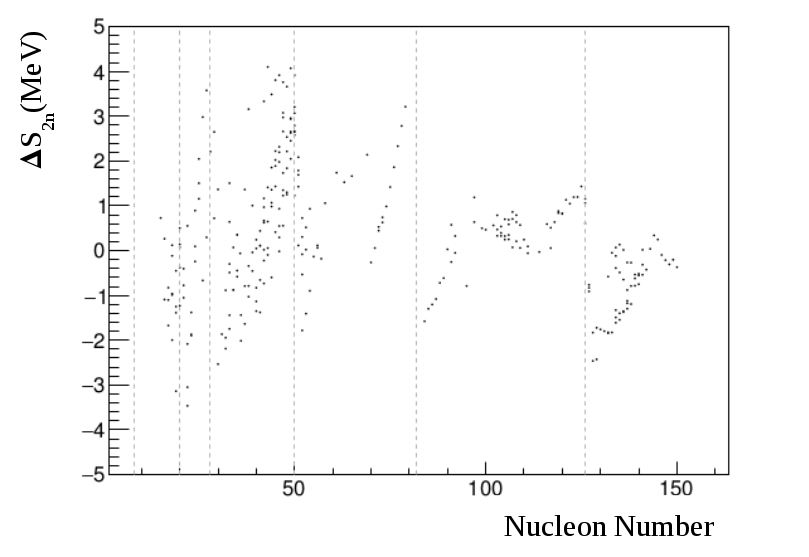
\includegraphics[width=\textwidth]{theory_two_neutron.png}
  \caption[The difference between the experimental two-neutron separation energy, $S_{2n}$, parsed from the evaluated nuclear data sheets \cite{EvittsParse} and the value obtained from the semi-empirical mass formula \cite{KraneText}.]{The difference between the experimental two-neutron separation energy, $S_{2n}$, parsed from the evaluated nuclear data sheets \cite{EvittsParse} and the value obtained from the semi-empirical mass formula \cite{KraneText}. The parameters used here are 15.5 MeV for the volume term, 16.8 MeV for the surface term, 0.72 MeV for the Coulomb term, 23 MeV for the symmetry term and 34 MeV for the pairing term \cite{KraneText}. The magic numbers of 8, 20, 28, 50, 82 and 126 are shown by the grey dashed lines where there are sudden drops. Image from \cite{EvittsThesis}.}
  \label{figure: two neutron separation energy plot}
\end{figure}

Characterization of the sequence of nuclear energy levels requires a treatment within the formalism of quantum mechanics. The nuclear potential is a combination of a strong force interaction between all nucleons, and a coulomb interaction between the positively charged protons \cite{CastenText}. The shear degree of inter-nucleon interaction terms that must be considered makes this an insoluble problem by explicit analytic means. As an approximation, the harmonic oscillator potential provides a reasonable starting point. The potential $V(r)$ is given by \cite{CastenText}

\begin{align}
	V(r) = \frac{1}{2}m\omega^2r^2
	\label{equation: harmonic oscillator potential}
\end{align}

where $m$ is the mass of the nucleon, $\omega$ is the oscillating frequency, and $r$ denotes the radius. Inserting this potential into the three-dimensional Schr\"odinger equation

\begin{equation}
\Bigg[\frac{-\hbar^2}{2m}\nabla^2+V(r)\Bigg]\Psi(r) = E\Psi(r)
\label{equation: 3D schrodinger}
\end{equation}

yields an analytic solution for the energy levels, as desired.  But this approximation fails to reproduce the characteristic magic numbers for nucleon shell closures, as observed experimentally. A more appropriate approximation can be made by modeling the nuclear potential as a mean field. This theoretical model replicates the approximate charge distribution of the nucleus, with the central region constant \cite{CastenText}. This potential, known as the Woods-Saxon potential, is of the form

\begin{equation}
V(r) = \frac{-V_0}{1+\mathrm{exp}[(r-R)/a]}
\label{equation: woods-saxon potential}
\end{equation}

where the strength of the potential is a function of r, the radial distance from the origin. $R = A^{1/3}\mskip\thinmuskip \mathrm{fm}$ is the mean radius of a nucleus, $A$ is the atomic mass number, $a=\SI{0.524}{fm}$ is the skin thickness (i.e. the radius of the nucleus in which the charge density decreases from $90\%$ of its value to $10\%$), and $V_0$ is an adjustable parameter in order to replicate the correct separation energies \cite{KraneText}. Additionally, a spin-orbit coupling force must be included in the potential. This force is an interaction between the intrinsic nuclear spin of the nucleon, and its orbital angular momentum. In short, increasing degree of alignment between the nucleon's spin and angular momentum will increase the attractiveness of the potential. Substituting this complete potential into the three-dimensional Schr\"odinger equation is capable of reproducing the magic numbers that we observe experimentally. The energy levels yielded by these subsequent approximation attempts are shown in Figure \ref{figure: energy level solutions for three potentials} \cite{KraneText}. An energy level is defined by the label ``$nl$" where $l$ is the orbital angular momentum denoted by a letter i.e. $s, \ p, \ d, \ f,$ corresponds to values 0, 1, 2, and 3 respectively. The number $n$ is an index denoting the $n^\mathrm{th}$ occurrence of a level with that particular $l$ value, starting from $n=0$. The parity of a state, $\pi$, is determined by $(-1)^l$. Each level can contain a maximum of 2(2$l$+1) nucleons, due to degeneracy of both $s$ and $m$, representing the spin and magnetic quantum numbers \cite{KraneText}.  

\begin{figure}[!ht]
  \centering
  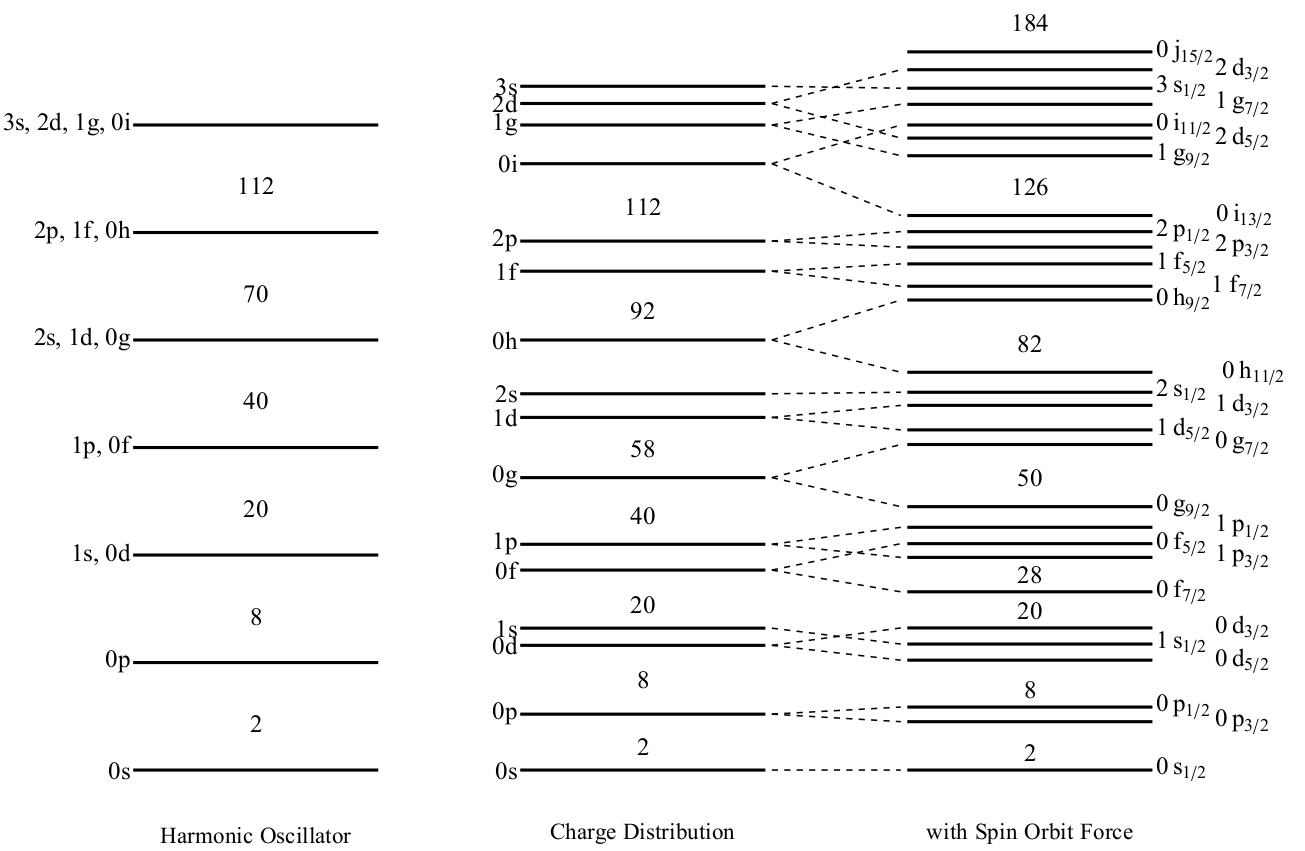
\includegraphics[width=\textwidth]{theory_schrodinger_energies.png}
  \caption[The energy levels yielded by solving the 3-D Schr\"odinger Equation (\ref{equation: 3D schrodinger}) for three different theoretical energy potential approximations: harmonic oscillator, Woods-Saxon, and Woods-Saxon with spin-orbit coupling.]{The energy levels yielded by solving the 3-D Schr\"odinger Equation (\ref{equation: 3D schrodinger}) for three different theoretical energy potential approximations: harmonic oscillator, Woods-Saxon, and Woods-Saxon with spin-orbit coupling. The number between particular levels is the number of nucleons required to fill a major shell. Only after the inclusion of the spin-orbit coupling interaction are the empirically observed magic numbers reproduced. Image from \cite{EvittsThesis}.}
  \label{figure: energy level solutions for three potentials}
\end{figure}

%%%%%%%%%%%%%%%%%%%%%%%%%%%%%%%%%%%%%%%%
\section{The Mixing of Nuclear States}
%%%%%%%%%%%%%%%%%%%%%%%%%%%%%%%%%%%%%%%%

Nuclei, being fundamentally quantum mechanical objects, exist in states that are best described as a linear combination of unperturbed states with equal spin and parity. Furthermore, there exists the potential for an interaction, $V$, between two mixed states. In Figure \ref{figure: diagram of two-state mixing model} two initial states are shown with energies $E_{1/2}$ and wavefunctions $\phi_{1/2}$. The interaction, $V$, between them results in a perturbation of their energies and wavefunctions. The resulting states are labelled by energies $E_{\mathrm{I/II}}$ and wavefunctions $\psi_{\mathrm{I/II}}$  \cite{KraneText}. 

\begin{figure}[!ht]
  \centering
  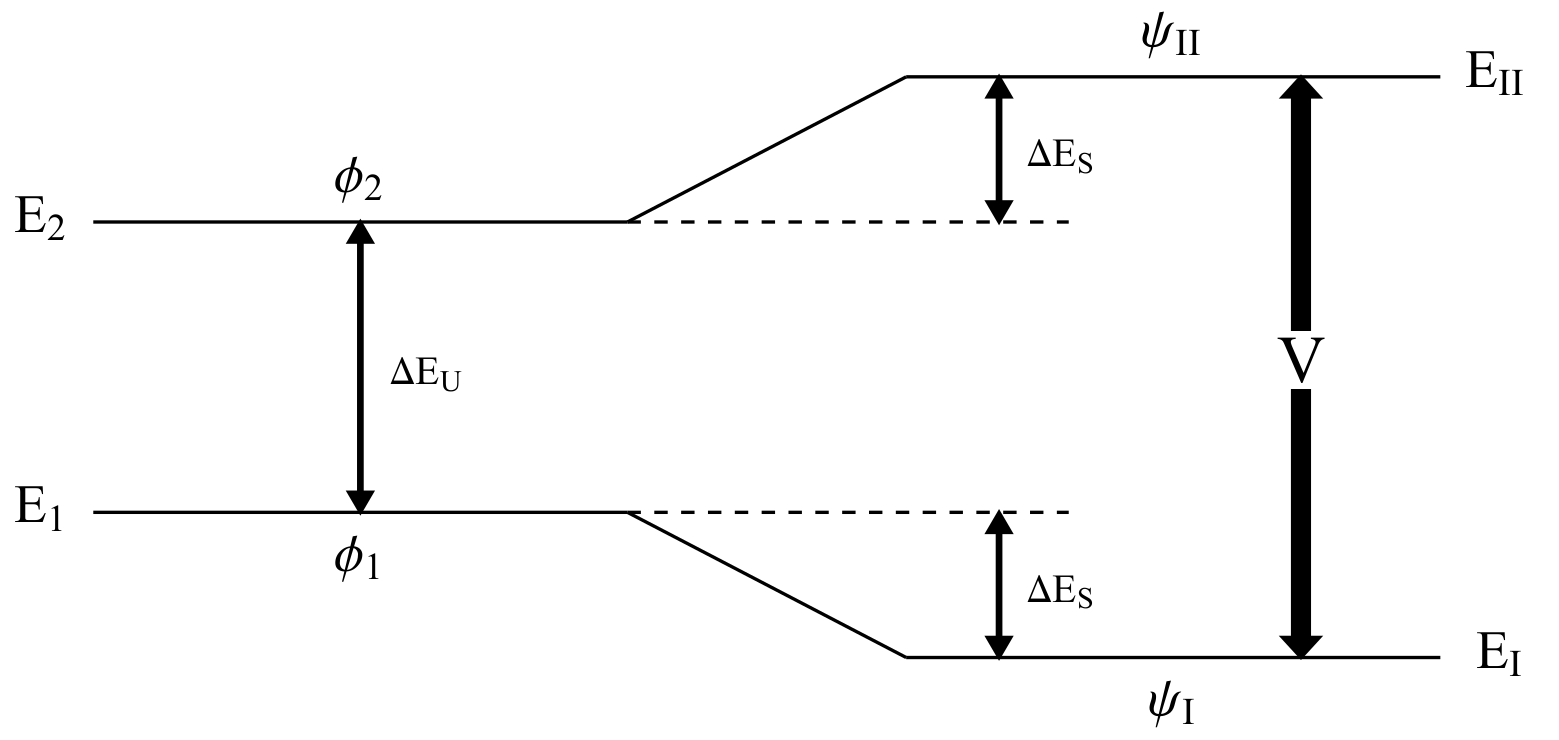
\includegraphics[width=\textwidth]{theory_mixing_diagram.png}
  \caption[Diagram of a two-state mixing interaction \cite{KraneText}. Image from \cite{EvittsThesis}.]{Diagram of a two-state mixing interaction \cite{KraneText}. Image from \cite{EvittsThesis}.}
  \label{figure: diagram of two-state mixing model}
\end{figure}

These new wavefunctions can be described by the degree of mixing that occurs between the original states. In the following expressions:

\begin{equation}
\begin{aligned}
\psi_\mathrm{I} = & a\phi_1 + b\phi_2 \\
\psi_\mathrm{II} = & -b\phi_1 + a\phi_2 \\
\label{equation: wavefunctions of mixed states}
\end{aligned}
\end{equation}

where $a$ and $b$ are the mixing amplitudes with normalization such that $a^2 + b^2 = 1$. If we consider the wavefunctions of the two unperturbed states, $\phi_{1/2}$, within energy space, then the closer the energies of these two states are, the greater degree of overlap will exist between the two wavefunctions. Hence, the strength of the mixing is a function of both the size of the interaction, $V$, and the size of the gap between the two energies, $E_{1/2}$. The ratio $R = \Delta E_\mathrm{U}/V$ encapsulates these two contributions, where $E_\mathrm{U}$ is the unperturbed energy difference as pictured in Figure \ref{figure: diagram of two-state mixing model} \cite{CastenText}. The energy difference following the interaction perturbation, $E_\mathrm{P}$, can be related to to $E_\mathrm{U}$ and $R$ by

\begin{equation}
\frac{\Delta E_\mathrm{P}}{\Delta E_\mathrm{U}} = \sqrt{1+\frac{4}{R^2}}
\label{equation: two state mixing energy gaps and strength}
\end{equation}

and the total shift in energy undergone by one of the states, $\Delta E_\mathrm{S}$, is given by

\begin{equation}
\frac{\lvert \Delta E_\mathrm{P} \rvert}{\Delta E_\mathrm{U}} = \frac{1}{2}\Bigg[\sqrt{1+\frac{4}{R^2}}-1\Bigg]
\label{equation: two state mixing - single state energy shift}
\end{equation}

A lower limit on the mixing amplitude $b$ can be expressed in terms of the ratio, $R$, as follows

\begin{equation}
b = \frac{1}{\sqrt{1+\Big[R/2+\sqrt{1+R^2/4}\Big]^2}}
\label{equation: two state mixing - amplitude b in terms of R}
\end{equation}

An interpretation of mixing as it relates to the two aforementioned physical contributions, unperturbed energy gap and interaction magnitude, can be gleaned from this expression. As the energy gap between the unperturbed states is increased relative to the interaction strength, the resulting $R$ value becomes large. Substituted into Equations (\ref{equation: two state mixing - single state energy shift}) and (\ref{equation: two state mixing - amplitude b in terms of R}) yields small values of $b$ and $\Delta E_\mathrm{S}$. With a negligible $\Delta E_\mathrm{S}$ value, Equation (\ref{equation: two state mixing - amplitude b in terms of R}) becomes purely a function of the interaction strength, $V$, i.e. it becomes possible to calculate $V$ from an experimental measurement of $b$. In the inverse situation, with large interaction and small unperturbed energy gap (i.e. $\Delta E_\mathrm{U} \approx 0$) then the states following the consideration of mixing become $E_\mathrm{I/II} = E_0 + V$, where each state is merely shifted from its initial energy, $E_0$, by the interaction strength only. This demonstrates that in any two-state mixing scenario, the observed energy difference between the two states may never be smaller than twice the interaction strength \cite{CastenText}. 

%%%%%%%%%%%%%%%%%%%%%%%%%%%%%%%%%%%%%%%%
\section{Collective Models of Nuclear Structure}
%%%%%%%%%%%%%%%%%%%%%%%%%%%%%%%%%%%%%%%%

While the nuclear shell model is an appropriate approximation for nuclei that have closed shells, it begins to lose applicability as the number of valence nucleons increases. For these regions an alternative model may be used that focuses on the collective nature of the nucleus. In non-spherical nuclei the deformation parameter, $\beta$ may be related to the eccentricity of the ellipsoid by

\begin{gather}
\beta = \frac{4}{3}\sqrt{\frac{\pi}{5}}\frac{\Delta R}{R_{\mathrm{AVG}}}
\label{equation: beta and spheroids}
\end{gather}

where $\Delta R$ is the difference between the semi-major and semi-minor axes of the ellipsoid and $R_\mathrm{AVG}=1.3A^{1/3} \si{fm}$, with $A$ being the atomic mass number. When $\beta>0$ the nucleus is prolate, and when $\beta<0$ the nucleus is oblate \cite{KraneText}. The excitation energies of an idealized deformed, axially-symmetric rotating nucleus are given be

\begin{gather}
E = \frac{\hbar^2}{2I}J(J+1)
\label{equation: rotational energies as function of J}
\end{gather}

where $I$ is the moment of inertia. The addition of rotational energy results in higher excited states with larger spin. Equation (\ref{equation: rotational energies as function of J}) is used to determine the idealized excitation energies of higher lying states; for example, in a nucleus of even number of protons and even number of neutrons the ground state is $0^+$ and the energies are

\begin{equation}
\begin{aligned}
E(0^+) ={} & 0 \\
E(2^+) ={} & 6(\hbar/2I) \\
E(4^+) ={} & 20(\hbar/2I)
\label{equation: three rotational energies calculated}
\end{aligned}
\end{equation}

Thus, the ratio of $4^+_1/2^+_1$ energies in a rigidly-deformed rotational nucleus is 3.33. Only even values of $J$ are considered due to the coupling of an even number of spins within the nucleus \cite{KraneText}. Generally, the ratio of $4^+_1/2^+_1$ energies is an indication of the macroscopic behaviour of the nucleus. In the regions between closed shells, this ratio ranges from 3.33 in rotational nuclei to 2.0 for nuclei that behave as spherical vibrators. Nuclei with intermediate values are described as the transitional nuclei between these two idealized cases. A chart of the nuclides is shown in Figure \ref{figure: 4 to 2 ratio across the chart} which displays the ratio of $4^+_1$ to $2^+_1$ energies. The magic numbers are highlighted as grey dashed lines. Red points correspond to a spherical vibrator where the ratio is close to 2.0 and the blue points are rotational nuclei where the ratio approaches 3.33. In the intermediate yellow region, a gradient of different configurations exists which are referred to as transitional nuclides. It can generally be concluded from Figure \ref{figure: 4 to 2 ratio across the chart} that the rotational nuclei exist in the regions between closed shells whereas the spherical vibrator nuclei are low mass (commensurate with low total nucleon number) or close to the magic numbers \cite{EvittsParse}. 

\begin{figure}[!ht]
  \centering
  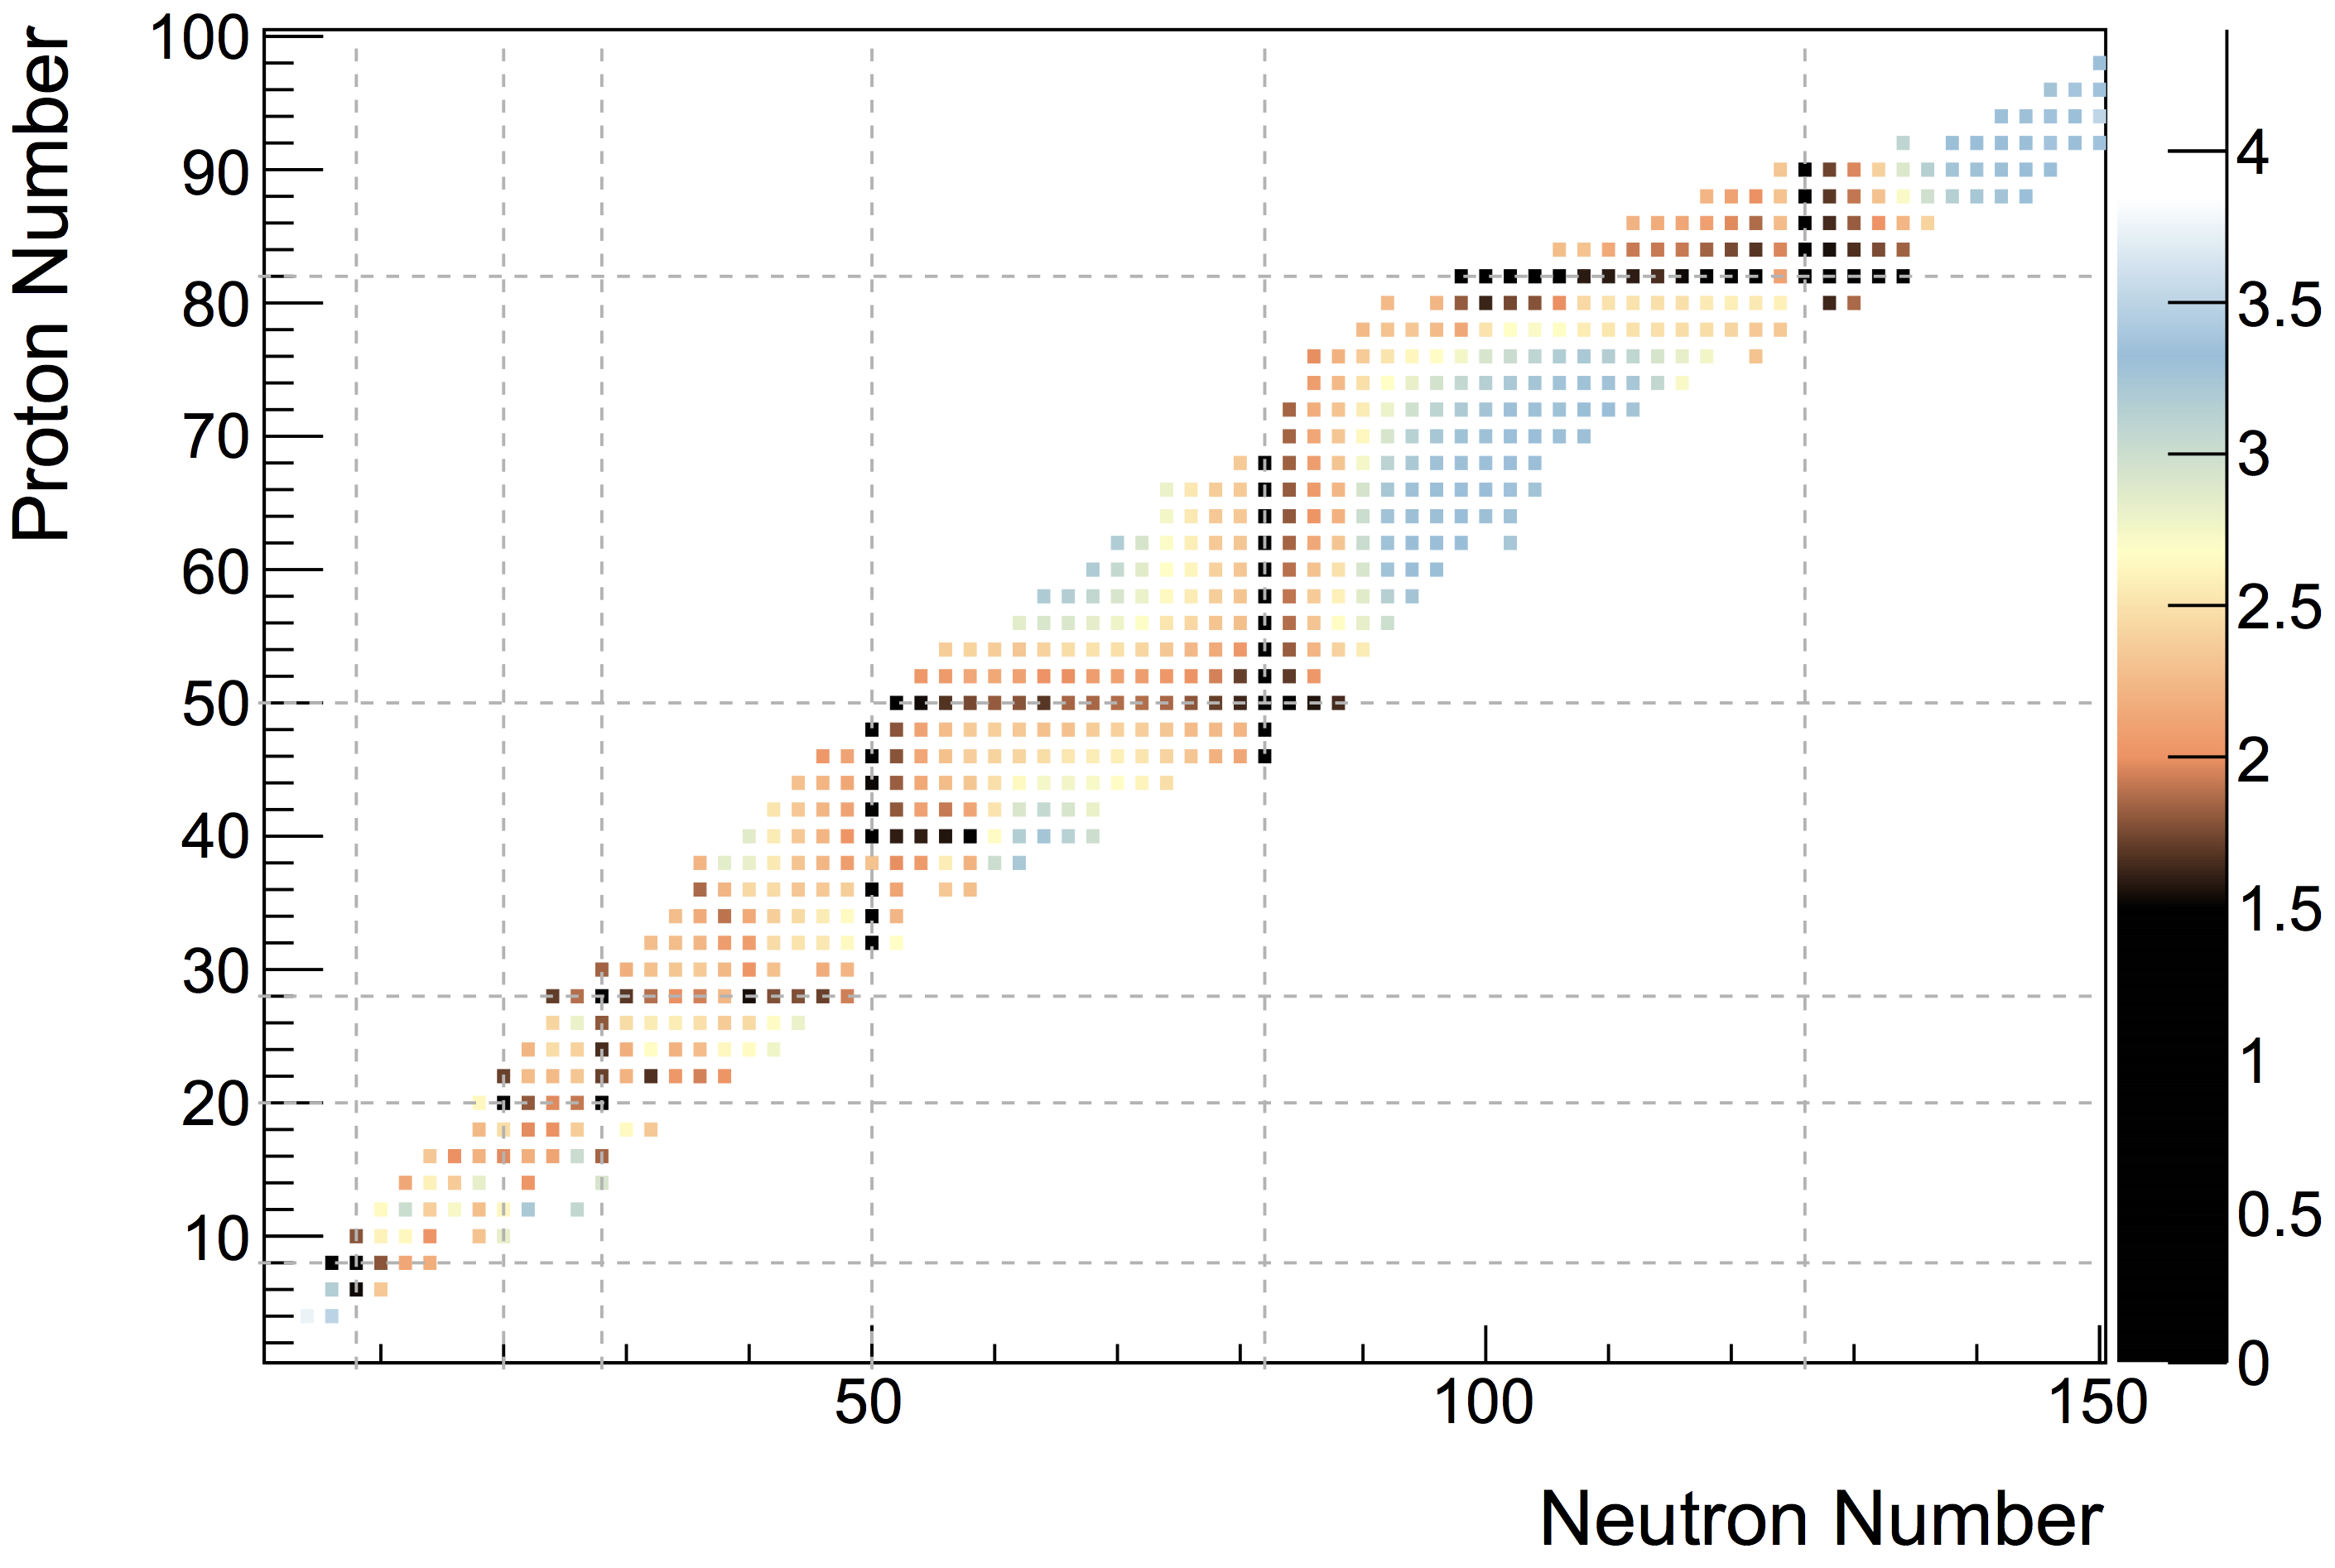
\includegraphics[width=\textwidth]{theory_4to2_chart.png}
  \caption[The ratio of $4^+_1$ to $2^+_1$ empirical energies for each nuclide across the chart \cite{EvittsParse}.]{The ratio of $4^+_1$ to $2^+_1$ empirical energies for each nuclide across the chart \cite{EvittsParse}. The magic numbers are shown by grey dashed lines. The red points correspond to a spherical vibrator, the blue are rotational, and the yellow are the transitional nuclei between the two. Image from \cite{EvittsThesis}.}
  \label{figure: 4 to 2 ratio across the chart}
\end{figure}

%%%%%%%%%%%%%%%%%%%%%%%%%%%%%%%%%%%%%%%%
\subsection{Shape Coexistence}
%%%%%%%%%%%%%%%%%%%%%%%%%%%%%%%%%%%%%%%%

The phenomenon of shape coexistence refers to a quantum mechanical behaviour, where a single nucleus simultaneously inhabits two or more possible configurations. Recalling the two-state mixing model, when two nuclear states of the same spin and parity (with similar excitation energies) but two different intrinsic shapes exist as an admixture, we can describe the situation as one of shape coexistence. 

If all possible configurations of nucleons within the nuclear volume are considered, and for each such configuration the inter-nuclear energy potential is plotted, then an energy potential surface is developed. In Figure \ref{figure: famous Pb figure} such a potential energy surface is plotted for the spin-zero states of the nucleus $^{186}\mathrm{Pb}$ \cite{Duguet2003}. The degree of spheroid deformation, expressed in terms of the parameter $\beta$ discussed earlier, varies along the $x$ and $y$ axes. The corresponding energy potential within the nucleus is plotted as the height, $z$. Hence, we see three distinct minima in the potential surface, each representing a potential nuclear shape that is part of the coexisting admixture. 

\begin{figure}[!ht]
  \centering
  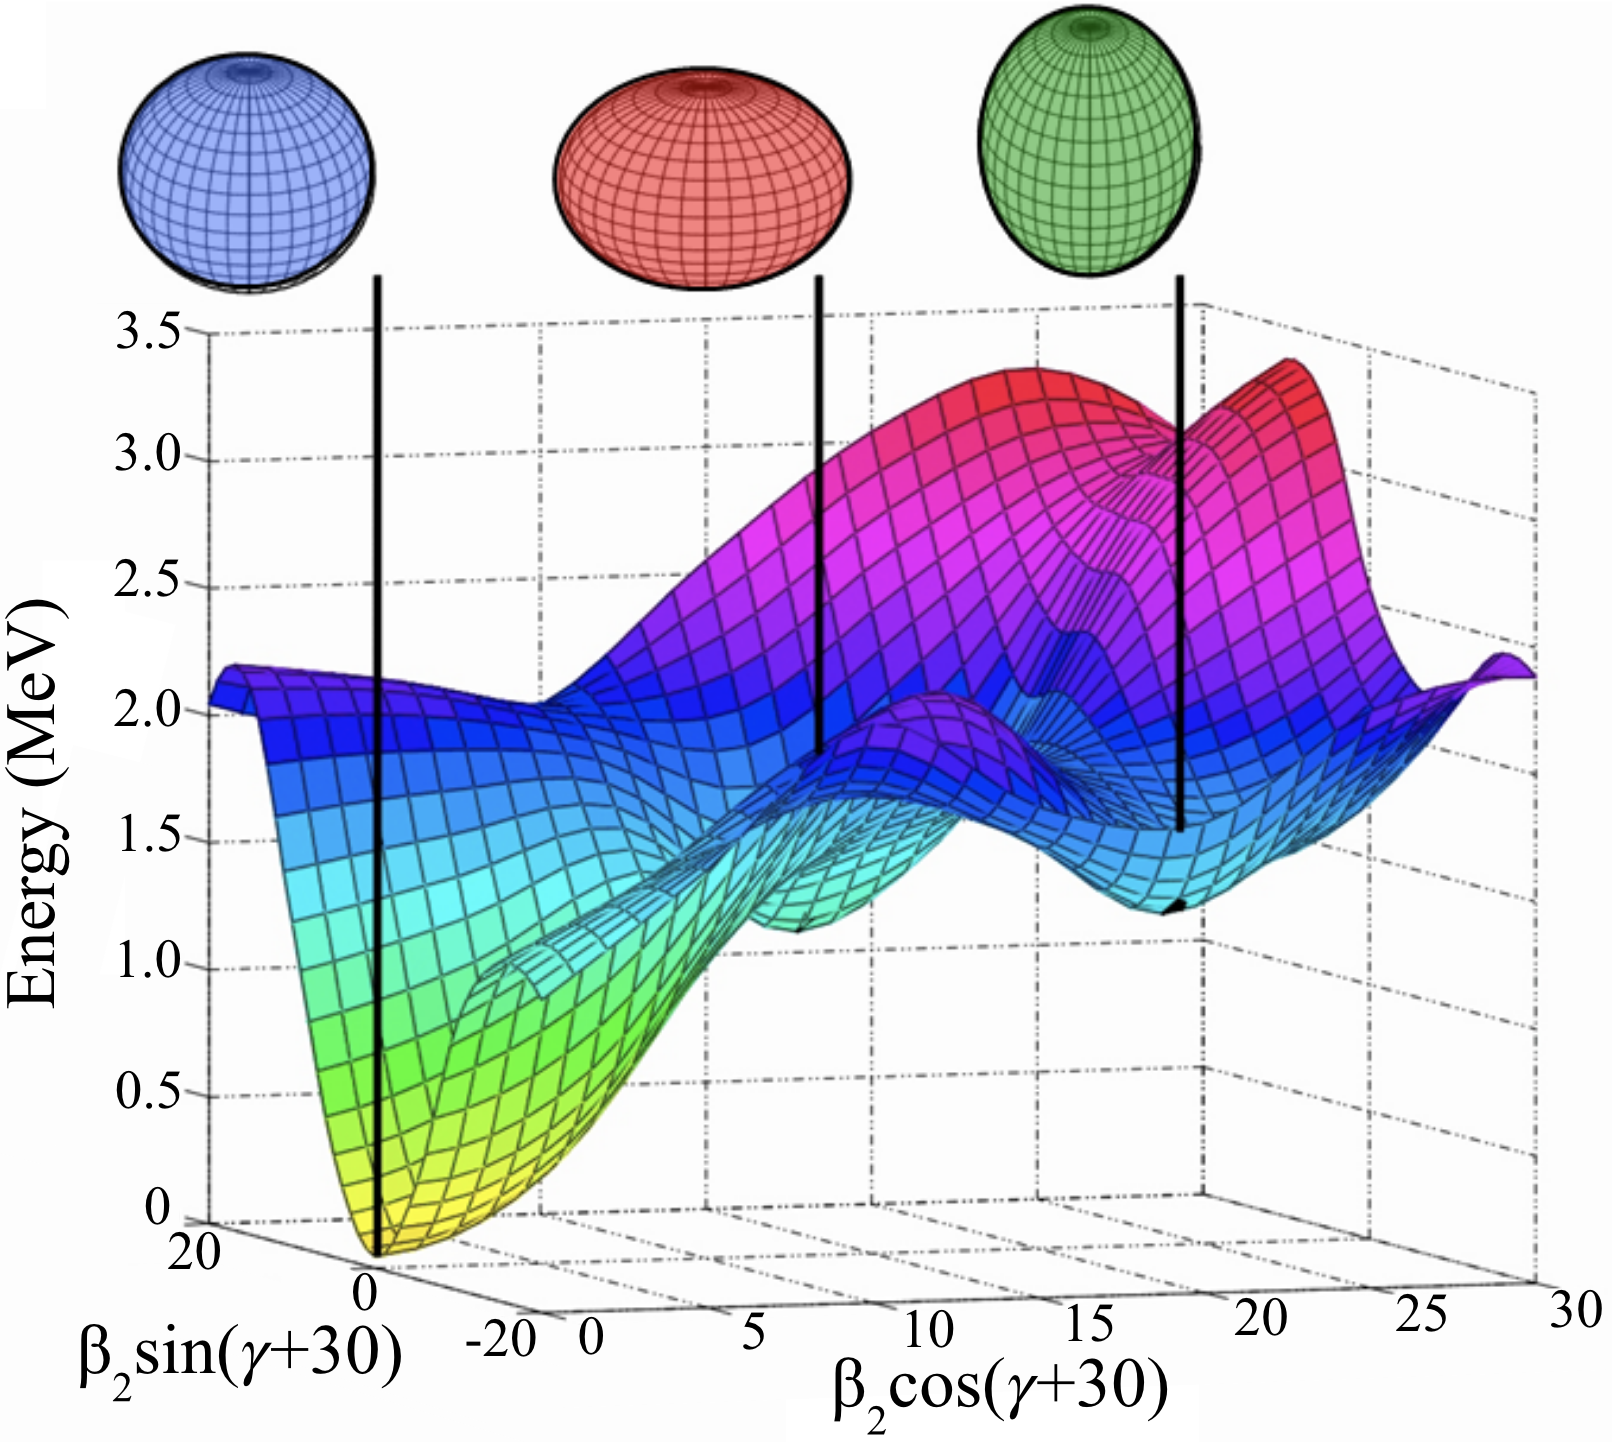
\includegraphics[width=0.7\textwidth]{theory_Pb_shape.png}
  \caption[The potential energy surface for $^{186}\mathrm{Pb}$ is plotted as a function of nuclear shape deformation. Three distinct minima, corresponding to three distinct nuclear structures, are highlighted.]{The potential energy surface for $^{186}\mathrm{Pb}$ is plotted as a function of nuclear shape deformation. The $x$ and $y$ axes correspond to deformations along the spheroid axes, in turn corresponding to reconfigurations of the constituent nucleons. The $\gamma$ parameter relates to the degree of triaxiality in the deformation (that is, the relative lengths of the three principal axes of the spheroidal nucleus). Three differently shaped spin-zero states are denoted by three distinct minima in the potential energy surface \cite{Duguet2003}.}
  \label{figure: famous Pb figure}
\end{figure}

%%%%%%%%%%%%%%%%%%%%%%%%%%%%%%%%%%%%%%%%
\section{Nuclear Reactions}
%%%%%%%%%%%%%%%%%%%%%%%%%%%%%%%%%%%%%%%%

Following a nuclear interaction, a nucleus can be left in a number of excited energy states. The reaction typically achieves a transfer of energy to the nucleus as part of a collision. These collisions can be categorized based on the degree of inter-penetration of the interacting nuclear volumes, which then corresponds to the force mechanism by which the interaction is mediated. In a collision where the colliding nuclei interact only electromagnetically, that is their position wavefunctions do not breach the short range within which the strong force applies, then the interaction mechanism is purely that of coulomb excitation. The nuclei themselves cannot be constitutively changed by this type of collision. In a pure Coulomb interaction, the interacting nuclei have only the possibility of being excited into low-lying energy states by the electromagnetic field. 

A nuclear collision that occurs at high enough energy such that strong force interactions occur, where the pure-coulomb interaction range is exceeded, is described as a ``beyond-barrier" collision. The interaction of the strong force from the different nucleons can lead to constitutive changes in nuclear structure, and not only are nuclei excited to higher lying states, but they also can exchange particles. 

From an experimental perspective, there are trade-offs between the different methods of populating the excited states of nuclei, dependent upon the desired observables for measurement. 

%%%%%%%%%%%%%%%%%%%%%%%%%%%%%%%%%%%%%%%%
\section{Gamma Decay}
%%%%%%%%%%%%%%%%%%%%%%%%%%%%%%%%%%%%%%%%

When excited nuclear states decay, they do so through transitions involving energy emission. The energy emitted from the nucleus may be in the form of photons, or particles. The dominant way that this occurs is through the emission of $\gamma$ rays. An emitted $\gamma$ ray will carry away energy equal to the difference in energy between the initial and final states of the transition. The emitted gamma rays can be characterized by the electromagnetic multipolarity of the associated transition. These multipolarities define the angular momentum, parity and angular distribution of the gamma ray emission in space. The angular momentum of the nuclear transition, and subsequently the $\gamma$ ray emitted, is governed by a set of selection rules, in conjunction with the parity \cite{KraneText}.

If the spin and parity of the two nuclear energy levels is given by $J^{\pi_i}_{i}$ and $J^{\pi_f}_{f}$, then the angular momentum carried away by the $\gamma$ ray, $L$, can take values in the following range

\begin{equation}
|J_i-J_f|\leq L \leq J_i+J_f
\label{equation: gamma ray decay vector difference}
\end{equation}

Additionally, $\gamma$ rays must carry away at least 1 $\hbar$ unit of angular momentum, thus forbidding gamma ray emission as a mechanism for transitions between two nuclear states of spin-0. Transitions of this nature must occur by other mechanisms, such as internal conversion electrons or internal pair formation \cite{KraneText}. 
Electromagnetic multipole fields are classified as either electric or magnetic in nature according to specific parity rules. If an electric transition has even $L$ then there is no change in parity but if $L$ is odd then there is a change in parity. The inverse rule defines magnetic transitions. i.e.

\begin{equation}
\begin{aligned}
&\pi(EL)=(-1)^{L} \\
&\pi(ML)=(-1)^{L+1}
\label{equation: gamma ray decay selection rules}
\end{aligned}
\end{equation}

Combined, these selection rules define the allowed multipolarities for a given transition. For example, in a $2^+$ to $2^+$ transition, the $M1$, $E2$, $M3$ and $E4$ processes will all have non-zero probability. There is also the $E0$ transition available but this will not decay through the emission of a $\gamma$ ray and will instead decay through alternate methods such as internal conversion \cite{KraneText}. 

%%%%%%%%%%%%%%%%%%%%%%%%%%%%%%%%%%%%%%%%
\section{Internal Conversion Decay}
%%%%%%%%%%%%%%%%%%%%%%%%%%%%%%%%%%%%%%%%

$E0$ transitions cannot occur by $\gamma$ ray emission due to the requirement for the photon to carry at least one unit of angular momentum. These transitions must occur by alternate modes, such as the emission of two photons ($\gamma \gamma$), production of an electron-positron pair (internal pair formation, $\pi$), or internal conversion electron decay.
In internal conversion electron decay, energy is released via the emission of one of the orbital electrons, with energy equal to the transition energy less the binding energy of the particular atomic orbital, $B_e$, i.e.

\begin{gather}
T_e = T_\gamma - B_e
\label{equation: icc conservation of energy}
\end{gather}

The total decay probability of a nuclear transition is equal to the sum of probabilities for the individual decay modes i.e.

\begin{gather}
\lambda_t = \lambda_\gamma + \lambda_e + \lambda_{\gamma \gamma} + \lambda_\pi +...
\label{equation: total decay as constituent sum}
\end{gather}

This can be rearranged as

\begin{gather}
\lambda_t = \lambda_\gamma(1+\alpha_e+\alpha_{\gamma \gamma}+ \alpha_\pi+...)
\label{equation: re-arrange to define alpha icc}
\end{gather}

where $\alpha_x=\lambda_x/\lambda_\gamma$ is the coefficient of the specific decay mode, defined as a probability of that mode relative to $\gamma$ ray decay. $\alpha_e$ is the internal conversion coefficient \cite{KraneText}.

%%%%%%%%%%%%%%%%%%%%%%%%%%%%%%%%%%%%%%%%
\section{$E0$ Transitions}
%%%%%%%%%%%%%%%%%%%%%%%%%%%%%%%%%%%%%%%%

Examination of the individual strength of an $E0$ transition requires that the different transition multipolarities be deconvolved. The two dominant transition multipolarities present in a $2^+ \rightarrow 2^+$ transition are $M1$ and $E2$. The mixing ratio, $\delta(E2/M1)$, is defined such that the intensities of these multipolarities can be obtained from 

\begin{gather}
\lambda(E2) = \frac{\delta^2}{1+\delta^2} \\
\lambda(M1) = \frac{1}{1+\delta^2}
\label{equation: disambiguating the mixing ratio}
\end{gather} 

The $(E2/M1)$ mixing ratio and the internal conversion coefficient are both required for the calculation of $q^2$, which is the ratio of intensities between $E0$ and $E2$ transitions from a common initial state. It is given by $q^2 = I(E0)/I(E2)$. For a $2^+\rightarrow2^+$ transition, the mixing of $E0$, $M1$ and $E2$ components (higher $L$ components may be neglected) results in a $q^2$ determined by

\begin{gather}
q^2 = \frac{\alpha_\mathrm{exp}(1+\delta^2)-\alpha(M1)}{\alpha(E2)\cdot \delta^2}-1
\label{equation: squared}
\end{gather}

where $\alpha$ are theoretical conversion coefficients obtained from BrIcc \cite{KIBEDI2008202}, and $\alpha_\mathrm{exp}$ is an experimentally determined value of the internal conversion coefficient (i.e. ratio of $E0+M1+E2$ electrons vs. $M1+E2$ $\gamma$ rays). Using all of the available experimental inputs such as $q^2$, $\delta$, branching ratios and parent half-lives, then $\rho^2(E0)$ may be calculated from

\begin{gather}
\rho^2(E0) = \frac{1}{\Omega(E0) \cdot \tau(E0)}
\label{equation: E0 strength}
\end{gather}

where $\Omega$ is an electronic factor and $\tau(E0)$ is the partial mean lifetime of the $E0$ transition \cite{KIBEDI2008202}. 

The $E0$ transition strength can also be expressed in terms of the degree of mixing between different, coexisting shape states of the nucleus. Its sensitivity to shape coexistence in nuclei is best represented in  the following expression \cite{Wood1999}

\begin{gather}
\rho^2(E0) = \frac{Z^2}{R_0^4}a^2(1-a^2)\Big[\Delta \langle r^2 \rangle \Big]^2
\label{equation: E0 as probe of shape coexistence}
\end{gather}

where $Z$ is the proton number of the nucleus, $R_0$ is the nuclear radius of its hypothetical spherical configuration, $a$ is the degree of mixing between two possible states, and $\Delta \langle r^2 \rangle$ is the difference in the root-mean-squared charge radius of the two coexisting configurations. This gives the relevance of $\rho^2(E0)$ measurements explicitly within the terms of the nuclear structure context as developed thus far. 

\endinput

Any text after an \endinput is ignored.
You could put scraps here or things in progress.

% \begin{gather}
% \rho^2(E0) = q^2 \times \frac{\alpha_K(E2)}{\Omega_K(E0)} \times \frac{BR(E2_\gamma)}{\tau}
% \end{gather}
% where $\Omega_K(E0)$ is an electronic factor from atomic theory, $\tau$ is the lifetime of the parent state, and $BR(E2_\gamma)$ is the branching ratio of the $E2$ $\gamma$ ray transition. These latter two components are known values available on NNDC [!!! cite].

% \begin{gather}
% \tau(E0) = \frac{\Sigma \lambda_r}{\lambda_r(E0)}\cdot\tau
% \label{partialLifetime}
% \end{gather}
% where $\lambda_r$ is a relative decay constant and $\tau=T_{1/2}/\mathrm{ln}(2)$; $T_{1/2}$ is the half-life. \cite{KraneText}. This calculation requires a summation over every available decay mode from the parent state. 

\begin{equation}
\begin{aligned}
A_\eta(J_i L_1 L_2 J_f) ={} & \frac{1}{1+\delta^2}[f_\eta(J_f L_1 L_1 J_i)+ \\
					     & 2\delta f_\eta (J_f L_1 L_2 J_i)+     \\
                         & \delta^2 f_\eta (J_f L_2 L_2 J_i)]
\end{aligned}
\label{equation: angular distribution coefficient}
\end{equation}



